\documentclass[12pt,a4paper]{report}

% =========================================================
% BookVault — Rapport Intergiciel (Overleaf-ready)
% Images : placer les .png/.jpg dans le même dossier que ce .tex (ou adapter les chemins).
% Filigrane : bookvaulticon.png (RGBA, fond transparent).
% Figures : architecture_microservices.png, bukvault-MCD.png, flux_inscription_utilisateur.png, …
% =========================================================

\usepackage[T1]{fontenc}
\usepackage[utf8]{inputenc}
\usepackage[french]{babel}

\usepackage{geometry}
\geometry{a4paper, margin=1.5cm}

\usepackage{graphicx}
\usepackage{float}
\usepackage{booktabs}
\usepackage{longtable}
\usepackage{array}
\usepackage{caption}
\usepackage{subcaption}
\usepackage{xcolor}
\usepackage{hyperref}
\usepackage{url}
\usepackage{csquotes}
\usepackage{listings}
\usepackage{titlesec}
\usepackage{enumitem}
\usepackage{fancyhdr}
\usepackage{eso-pic}
\usepackage{tikz}

% --- Filigrane BookVault (logo centré, opacité réduite) ---
% Sur Overleaf : copier bookvaulticon.png à côté du .tex OU garder le chemin ci-dessous.
\newcommand{\bookvaulticonpath}{bookvaulticon.png}
% Overleaf (fichier à la racine du projet) : \renewcommand{\bookvaulticonpath}{bookvaulticon.png}
\newcommand{\bookvaultWatermarkOpacity}{0.08}   % 0.08--0.15 : ajuster si trop visible
\newcommand{\bookvaultWatermarkWidth}{0.72\paperwidth}

\newcommand{\BookVaultWatermark}{%
  \AddToShipoutPictureBG{%
    \begin{tikzpicture}[remember picture,overlay]
      \node[opacity=\bookvaultWatermarkOpacity,inner sep=0pt] at (current page.center) {%
        \includegraphics[width=\bookvaultWatermarkWidth]{\bookvaulticonpath}%
      };
    \end{tikzpicture}%
  }%
}

\hypersetup{
  colorlinks=true,
  linkcolor=blue!50!black,
  urlcolor=blue!50!black,
  citecolor=blue!50!black,
  pdftitle={BookVault — Rapport Intergiciel},
  pdfauthor={BookVault Team},
  pdfsubject={Architecture microservices, intergiciel, frontend Angular},
}

\setlist{itemsep=2pt, topsep=4pt}

\lstdefinestyle{bookvault}{
  basicstyle=\ttfamily\small,
  breaklines=true,
  frame=single,
  framerule=0.2pt,
  rulecolor=\color{black!20},
  backgroundcolor=\color{black!2},
  keywordstyle=\color{blue!60!black},
  commentstyle=\color{green!40!black},
  stringstyle=\color{red!50!black},
  showstringspaces=false
}
\lstset{style=bookvault}

\pagestyle{fancy}
\fancyhf{}
\lhead{BookVault}
\rhead{Rapport Intergiciel}
\cfoot{\thepage}

% Chapitres : I. Introduction (romains, sans « Chapitre »)
\renewcommand{\thechapter}{\Roman{chapter}}
\renewcommand{\chaptername}{}
\titleformat{\chapter}[hang]
  {\normalfont\huge\bfseries}
  {\thechapter.}
  {0.6em}
  {}
\titlespacing*{\chapter}{0pt}{3.5ex plus 1ex minus .2ex}{2.3ex plus .2ex}
\titlecontents{chapter}[0pt]%
  {\addvspace{1ex}\bfseries}%
  {\thecontentslabel.\ }%
  {}%
  {\titlerule*[0.5pc]{.}\contentspage\par\vspace{0.5ex}}

% Sections / sous-sections : numérotation arabe seule (1, 1.1…), sans I., II.…
\renewcommand{\thesection}{\arabic{section}}
\renewcommand{\thesubsection}{\thesection.\arabic{subsection}}
\renewcommand{\thesubsubsection}{\thesubsection.\arabic{subsubsection}}
\AtBeginDocument{%
  \renewcommand{\theHsection}{\thechapter.\arabic{section}}%
  \renewcommand{\theHsubsection}{\thechapter.\thesubsection}%
  \renewcommand{\theHsubsubsection}{\thechapter.\thesubsubsection}%
}

\title{
  \textbf{BookVault}\\
  \large Plateforme modulaire distribuée (microservices)\\
  \vspace{0.8em}
  \normalsize Rapport d'implémentation Intergiciel\\
}
\author{
  Semestre 2 — Intergiciel\\
  \textit{Université / Établissement : \underline{\hspace{6cm}}}\\
  \textit{Encadrant : \underline{\hspace{7cm}}}\\
  \textit{Étudiant : Asaph Kouokam Talla (et équipe si applicable)}
}
\date{\today}

% -----------------------------
% Sigles / acronymes (simple, sans makeglossaries)
% -----------------------------
\newcommand{\sigle}[2]{\textbf{#1} — #2\\}

\begin{document}
\BookVaultWatermark

\begin{titlepage}
  \centering
  \vspace*{2cm}
  {\Huge\bfseries BookVault\par}
  \vspace{0.6cm}
  {\Large Plateforme de livres numériques et physiques — architecture microservices\par}
  \vspace{1.2cm}
  {\Large\bfseries Rapport Intergiciel\par}
  \vspace{1.2cm}
  {\large\bfseries Travail réalisé par\par}
  \vspace{1.2cm}
  {\large KOUOKAM TALLA EUGENE ASAPH — CM-UDS-21SCI0021\par}
  \vspace{1.0cm}
  {\large DZOYEM TSOMENE MÉGANE — CM-UDS-25SCI0755\par}
  \vspace{1.0cm}
  {\large YONKEU CHUSI Silvère Valdexe — CM-UDS-25SCI0751\par}
  \vspace{1.0cm}
  {\large LAPEWE TCHEUFFA Kessy — CM-UDS-25SCI0760\par}
  \vspace{1.0cm}
  {\large TETDA NAOUSSI ULRICH — CM-UDS-22SCI1192\par}

  \vfill
  % {\large \today\par}
\end{titlepage}

\pagenumbering{roman}
\chapter*{Résumé}
BookVault est une plateforme de gestion et de distribution de livres (ebooks et ouvrages physiques) bâtie selon une \textbf{architecture modulaire et distribuée}. Le projet met en œuvre un \textbf{API Gateway}, une constellation de \textbf{microservices Spring Boot} (authentification, profils, catalogue, commandes, fichiers, lecture, avis, wishlist, notifications, communauté, auteur et administration), ainsi qu'un front-end \textbf{Angular}. L'enjeu principal est d'illustrer les concepts d'intergiciel : routage, communication inter-services, sécurité centralisée (JWT), séparation des responsabilités, et stratégies pragmatiques pour maintenir la productivité en environnement distribué (stubs configurables, migrations progressives, proxy front).\par

Les choix techniques présentés dans ce rapport montrent l'intérêt d'un \textbf{système modulaire} : évolution indépendante des domaines (catalogue, commandes, lecture), ajout progressif de capacités (OAuth Google, vérification e-mail, dashboards agrégés), et optimisation du cycle de développement grâce à une configuration locale (Docker Compose, seeds, scripts).\par

\chapter*{Abstract}
BookVault is a modular distributed platform for ebook and physical book management. It relies on a microservices architecture (Spring Boot) behind an API Gateway, with an Angular frontend. The project highlights middleware concerns: routing, inter-service communication, centralized security (JWT), separation of responsibilities, and pragmatic strategies for local development (configurable stubs, progressive schema updates, frontend proxy).\par

\tableofcontents
\listoffigures
\cleardoublepage

\chapter*{Liste des sigles et abréviations}
\sigle{API}{Application Programming Interface}
\sigle{BFF}{Backend For Frontend}
\sigle{CDC}{Change Data Capture}
\sigle{CI/CD}{Continuous Integration / Continuous Delivery}
\sigle{CORS}{Cross-Origin Resource Sharing}
\sigle{DTO}{Data Transfer Object}
\sigle{EDA}{Event-Driven Architecture}
\sigle{GIS}{Google Identity Services}
\sigle{HMAC}{Hash-based Message Authentication Code}
\sigle{HTTP}{Hypertext Transfer Protocol}
\sigle{JWT}{JSON Web Token}
\sigle{MCD}{Modèle Conceptuel de Données}
\sigle{MoMo}{Mobile Money}
\sigle{OAuth}{Open Authorization}
\sigle{OIDC}{OpenID Connect}
\sigle{OTLP}{OpenTelemetry Protocol}
\sigle{RBAC}{Role-Based Access Control}
\sigle{REST}{Representational State Transfer}
\sigle{SQL}{Structured Query Language}
\sigle{UI}{User Interface}
\sigle{2PC}{Two-Phase Commit}

\cleardoublepage
\pagenumbering{arabic}

% =========================================================
% 1. Introduction & concepts
% =========================================================
\chapter{Introduction}
\section{Contexte et objectif}
L'essor des plateformes numériques (lecture sur mobile, paiements instantanés, communautés en ligne) impose des architectures capables de \textbf{monter en charge}, d'\textbf{évoluer rapidement} et de \textbf{séparer les responsabilités}. BookVault répond à ces enjeux en proposant une plateforme intégrée (catalogue, commandes, fichiers, lecture, avis, wishlist, notifications, communauté) tout en conservant une structure modulaire.\par

L'objectif de ce projet intergiciel est double :
\begin{itemize}
  \item \textbf{Démontrer une architecture distribuée} de type microservices, avec sécurité et communication inter-services.
  \item \textbf{Mettre en évidence des techniques d'API} : DTOs stables, validation, RBAC, gestion des tokens, et patterns de communication entre services.
\end{itemize}

\section{Concepts clés (aperçu)}
Les notions d'intergiciel, de microservices, d'API REST, de JWT et de patterns distribués sont développées au \textbf{chapitre~\ref{ch:referentiel}} (définition, fonctionnement, puis application au projet). Ce chapitre d'introduction pose le périmètre fonctionnel et la motivation.\par

\section{Périmètre fonctionnel}
Le périmètre couvre :
\begin{itemize}
  \item \textbf{Auth} : inscription, connexion, refresh token, OAuth Google, vérification e-mail.
  \item \textbf{Users} : profils, rôles, paramètres lecteur.
  \item \textbf{Catalogue} : livres, catégories, statuts, visibilité, vues.
  \item \textbf{Fichiers} : upload/download (ebook, cover, avatar) et stockage.
  \item \textbf{Orders} : panier, commandes, paiement (références), lignes.
  \item \textbf{Reading} : progression, signets, annotations.
  \item \textbf{Reviews} : avis, helpful, signalements.
  \item \textbf{Wishlist} : favoris, déplacement vers panier.
  \item \textbf{Notifications} : préférences, notifications, abonnements livre.
  \item \textbf{Community} : hub, threads, événements, messagerie, likes, suggestions.
  \item \textbf{Admin/Auteur} : dashboards, file de validation, stats.
\end{itemize}

% =========================================================
% 2. Référentiel théorique des techniques
% =========================================================
\chapter{Référentiel théorique des techniques intergicielles}
\label{ch:referentiel}

Ce chapitre présente, pour chaque technique mobilisée dans BookVault, une \textbf{définition}, un \textbf{fonctionnement} (mécanisme général) puis l'\textbf{application concrète} au projet. L'ordre respecte la logique pédagogique de la soutenance : comprendre le concept avant la démonstration.

\section{Intergiciel (middleware)}

\paragraph{Définition.} Couche logicielle intermédiaire qui fournit des services transverses (communication, sécurité, routage, transformation, journalisation) entre applications hétérogènes, masquant la complexité du réseau et des protocoles.\par

\paragraph{Fonctionnement.} Les composants clients n'appellent pas directement chaque service métier : ils passent par des \textit{connecteurs} (gateway, bus de messages, proxies) qui appliquent des politiques communes (authentification, CORS, agrégation). L'intergiciel réduit le couplage entre producteurs et consommateurs de données.\par

\paragraph{Dans BookVault.} L'\textbf{API Gateway} Spring Cloud Gateway (port 8080) centralise l'entrée \texttt{/api/v1}. Les clients HTTP inter-services (\texttt{RestTemplate}/\texttt{WebClient}) et la configuration \texttt{*\_SERVICE\_URI} relient les microservices. Le proxy Angular en développement joue un rôle d'intergiciel côté front.\par

\paragraph{Références.} Documentation Microsoft Azure Architecture ; littérature SOA/ESB.\par


\section{Architecture microservices}

\paragraph{Définition.} Style architectural consistant à découper une application en \textbf{petits services autonomes}, chacun exécuté dans son propre processus, communiquant via des mécanismes légers (souvent HTTP/REST), déployables indépendamment et alignés sur des \textbf{capacités métier}.\par

\paragraph{Fonctionnement.} Les caractéristiques reconnues (Lewis \& Fowler) incluent : composantisation par services, organisation par capacités métier, \textit{smart endpoints and dumb pipes}, gouvernance décentralisée, \textbf{gestion des données décentralisée}, automatisation du déploiement, conception pour l'échec, design évolutif. Les transactions distribuées ACID globales sont évitées ; on privilégie la compensation et la cohérence éventuelle.\par

\paragraph{Dans BookVault.} BookVault compte une quinzaine de services (auth, user, catalog, order, file, reading, review, wishlist, notification, community, author, admin) + gateway. Chaque service possède son dépôt Maven et sa base PostgreSQL.\par

\paragraph{Références.} Martin Fowler, \textit{Microservices} ; James Lewis \& Martin Fowler, article original (2014).\par


\section{API Gateway}

\paragraph{Définition.} Point d'entrée \textbf{unique} et centralisé entre les clients (navigateur, mobile) et un ensemble de microservices. La gateway agit comme un \textbf{reverse proxy} conscient des API : elle route les requêtes, peut agréger des réponses et applique des préoccupations transverses (CORS, TLS, limitation de débit).\par

\paragraph{Fonctionnement.} Le client envoie une requête à une URL publique ; la gateway inspecte le chemin, les en-têtes et la méthode HTTP, puis la transmet au service cible selon des règles de routage. Elle peut aussi transformer les requêtes/réponses et masquer la topologie interne (adresses IP, ports). En architecture mature, elle gère le trafic \textit{north-south} (extérieur $\rightarrow$ système), tandis qu'un \textit{service mesh} peut gérer l'est-ouest (service $\rightarrow$ service).\par

\paragraph{Dans BookVault.} \texttt{api-gateway} route \texttt{/api/v1/auth/**} vers auth (8081), \texttt{/books/**} vers catalog (8083), etc. Les variables d'environnement (\texttt{CATALOG\_SERVICE\_URI}, \ldots) permettent le déploiement multi-PC. \texttt{GatewayCorsConfig} autorise le front Angular.\par

\paragraph{Références.} Microsoft Learn — API gateways ; Palo Alto Networks — What is an API Gateway.\par


\section{Database per service}

\paragraph{Définition.} Patron de persistance : chaque microservice \textbf{possède et gère exclusivement} ses données ; aucun autre service n'accède directement à sa base. L'accès inter-domaines se fait uniquement par \textbf{API} ou \textbf{événements}.\par

\paragraph{Fonctionnement.} On peut implémenter l'isolation à plusieurs niveaux : tables privées, schéma dédié, ou serveur PostgreSQL distinct par service. Les avantages : déploiement et migrations indépendants, choix technologique par service (\textit{polyglot persistence}), isolation des pannes. Les inconvénients : plus de jointures SQL cross-domaines ; transactions métier multi-services nécessitent Saga, outbox ou agrégation API.\par

\paragraph{Dans BookVault.} \texttt{bookvault\_catalog}, \texttt{bookvault\_order}, \texttt{bookvault\_auth}, etc. Les identifiants UUID (\texttt{userId}, \texttt{bookId}) servent de clés de corrélation. Les entitlements ebook passent par \texttt{order-service}, pas par lecture directe de sa base.\par

\paragraph{Références.} microservices.io — Database per service ; Microsoft .NET microservices docs.\par


\section{Communication synchrone HTTP}

\paragraph{Définition.} Mode d'intégration \textbf{requête-réponse} : le service appelant bloque jusqu'à la réponse du service appelé (ou timeout). Protocole courant : HTTP/1.1 ou HTTP/2 avec JSON.\par

\paragraph{Fonctionnement.} Le client HTTP construit une requête (méthode, URL, en-têtes, corps), ouvre une connexion TCP, attend la réponse, puis traite le code de statut et le corps. Les erreurs réseau, les lenteurs et les dépendances en chaîne augmentent la latence perçue et le risque de \textbf{cascade de défaillances} si un service aval est indisponible.\par

\paragraph{Dans BookVault.} \textit{order-service} $\rightarrow$ \textit{catalog-service} pour prix/disponibilité ; \textit{file-service} $\rightarrow$ \textit{order-service} pour entitlements ; \textit{wishlist-service} $\rightarrow$ \textit{order-service} pour ajout panier. Configuration via \texttt{order.catalog.base-url}, etc.\par

\paragraph{Références.} REST ; documentation Spring \texttt{RestTemplate}/\texttt{WebClient}.\par


\section{Architecture événementielle et Apache Kafka}

\paragraph{Définition.} L'\textbf{architecture événementielle} modélise les interactions par \textbf{événements} (faits métier immuables : \texttt{OrderPaid}, \texttt{BookPublished}) publiés sur un \textbf{broker} (Apache Kafka, RabbitMQ). Les producteurs ignorent les consommateurs ; les consommateurs réagissent de façon asynchrone.\par

\paragraph{Fonctionnement.} Un \textbf{topic} Kafka partitionne le flux d'événements pour le parallélisme. Les \textbf{producteurs} écrivent des enregistrements clé-valeur ; les \textbf{consommateurs} (souvent regroupés en \textit{consumer group}) lisent les partitions. Kafka persiste les messages sur disque (replay possible). La livraison est en général \textbf{au moins une fois} : les consommateurs doivent être \textbf{idempotents}.\par

\paragraph{Dans BookVault.} \textbf{Non implémenté} en V1 (pas de broker). Perspective : après \texttt{POST .../pay}, publier \texttt{OrderPaid} pour alimenter notifications, stats catalogue et badge « acheteur vérifié » sans coupler \textit{order} à \textit{review}.\par

\paragraph{Références.} Stack Overflow Blog — Event-driven topic design ; microservices.io — Idempotent consumer.\par


\section{Théorème CAP et cohérence}

\paragraph{Définition.} Dans un système de données \textbf{distribué}, on ne peut garantir simultanément plus de \textbf{deux} propriétés parmi : \textbf{C}onsistency (cohérence forte), \textbf{A}vailability (disponibilité), \textbf{P}artition tolerance (tolérance aux partitions réseau).\par

\paragraph{Fonctionnement.} Les partitions réseau étant inévitables, le choix se porte souvent entre cohérence et disponibilité \textbf{pendant} la panne. Un système \textbf{CP} refuse certaines écritures/lectures pour rester cohérent ; un système \textbf{AP} répond toujours mais peut renvoyer des données légèrement obsolètes (\textbf{cohérence éventuelle}). En pratique, les architectures modernes visent un compromis par opération (Brewer, 2012).\par

\paragraph{Dans BookVault.} BookVault privilégie disponibilité et isolation des domaines : notes moyennes, compteurs de vues et dashboards admin peuvent être \textbf{éventuellement cohérents}. Les stubs d'entitlement permettent le développement sans tous les services actifs.\par

\paragraph{Références.} Gilbert \& Lynch, preuve formelle ; Wikipedia — CAP theorem ; IBM Think — CAP.\par


\section{Pattern Backend for Frontend (BFF)}

\paragraph{Définition.} Patron où une \textbf{couche serveur dédiée} est créée pour chaque type d'expérience utilisateur (web, mobile, admin), plutôt qu'une API générique unique. Le BFF agrège, transforme et adapte les données des microservices au format attendu par le client.\par

\paragraph{Fonctionnement.} Le BFF appelle plusieurs services en parallèle, fusionne les réponses et renvoie une charge utile « prête pour l'UI ». Il doit rester \textbf{mince} : pas de logique métier dupliquée (celle-ci reste dans les microservices). Il se distingue de la gateway : la gateway route et sécurise globalement ; le BFF orchestre pour \textbf{un} client précis (Sam Newman, Microsoft Azure Patterns).\par

\paragraph{Dans BookVault.} \textit{admin-service} joue ce rôle : agrégation KPI, courbes de lecture, signalements en appelant user, catalog, reading, review — sans dupliquer leurs règles métier.\par

\paragraph{Références.} Sam Newman — Backends for Frontends ; Microsoft Learn — BFF pattern.\par


\section{REST (Representational State Transfer)}

\paragraph{Définition.} Style architectural défini par Roy Fielding (2000) pour les systèmes hypermédia distribués. Ce n'est pas un protocole ni un framework, mais un ensemble de \textbf{contraintes} visant performance, évolutivité et simplicité.\par

\paragraph{Fonctionnement.} Les six contraintes principales : (1) \textbf{interface uniforme} — manipulation de ressources via URI et représentations (JSON) ; (2) \textbf{client-serveur} — séparation des responsabilités ; (3) \textbf{sans état} — chaque requête contient toute l'information nécessaire (pas de session serveur) ; (4) \textbf{mise en cache} ; (5) \textbf{système en couches} (proxies, gateways) ; (6) \textbf{code à la demande} (optionnel). L'interface uniforme inclut l'usage des verbes HTTP (\texttt{GET}, \texttt{POST}, \texttt{PUT}, \texttt{PATCH}, \texttt{DELETE}) sur des ressources nommées.\par

\paragraph{Dans BookVault.} Toutes les API publiques sont sous \texttt{/api/v1}. Exemples : \texttt{GET /books}, \texttt{POST /cart/add}, \texttt{PATCH /notifications/\{id\}/read}. Le versionnement par préfixe prépare une future \texttt{v2}.\par

\paragraph{Références.} Fielding, thèse de doctorat, chapitre 5 ; restfulapi.net — REST constraints.\par


\section{DTO et validation Bean Validation}

\paragraph{Définition.} Un \textbf{DTO} est un objet (souvent immuable) transportant des données entre couches ou processus, sans logique métier. La \textbf{validation déclarative} (Jakarta Bean Validation : \texttt{@NotNull}, \texttt{@Size}, \texttt{@Email}) vérifie les contraintes avant l'exécution métier.\par

\paragraph{Fonctionnement.} Le contrôleur reçoit un DTO de requête annoté \texttt{@Valid} ; le framework valide et renvoie HTTP 400 si échec. La couche service manipule des entités JPA ; la couche API expose uniquement des DTOs de réponse, évitant les fuites (mot de passe, relations lazy).\par

\paragraph{Dans BookVault.} Records Java (\texttt{UserResponse}, \texttt{BookDetailResponse}) et types TypeScript (\texttt{api.types.ts}) alignés. Mot de passe inscription $\geq$ 8 caractères, notes avis 1--5, etc.\par

\paragraph{Références.} Patterns Enterprise Application ; documentation Jakarta Validation.\par


\section{Pagination et gestion d'erreurs API}

\paragraph{Définition.} La \textbf{pagination} découpe les grandes collections en pages (offset/limit ou curseur). La \textbf{gestion centralisée des erreurs} mappe les exceptions métier vers des codes HTTP et corps JSON homogènes.\par

\paragraph{Fonctionnement.} Spring Data \texttt{Pageable} accepte \texttt{page}, \texttt{size}, \texttt{sort} et renvoie \texttt{content}, \texttt{totalElements}, \texttt{totalPages}. Un \texttt{@ControllerAdvice} intercepte les exceptions (\texttt{NotFoundException} $\rightarrow$ 404, validation $\rightarrow$ 400) pour que le client ne parse pas une stack trace.\par

\paragraph{Dans BookVault.} Listes utilisateurs, livres, commandes, notifications paginées. Erreurs cohérentes pour le front Angular (toasts, messages utilisateur).\par

\paragraph{Références.} Documentation Spring Data REST ; RFC 7807 Problem Details (évolution possible).\par


\section{OpenAPI / Swagger}

\paragraph{Définition.} Standard (ex-Swagger) décrivant de façon machine-readable les endpoints, paramètres, schémas et codes de réponse d'une API REST. Swagger UI génère une documentation interactive.\par

\paragraph{Fonctionnement.} Le fichier OpenAPI (YAML/JSON) sert de \textbf{contrat} entre équipes front et back. Les clients peuvent générer du code ; les tests de contrat vérifient que l'implémentation respecte la spec (springdoc-openapi intègre cela à Spring Boot).\par

\paragraph{Dans BookVault.} Chaque microservice peut exposer \texttt{/swagger-ui.html} via springdoc. Utile en soutenance pour montrer les contrats sans lire le code Java.\par

\paragraph{Références.} OpenAPI Initiative ; springdoc-openapi documentation.\par


\section{JWT (JSON Web Token)}

\paragraph{Définition.} Standard ouvert pour transmettre des \textbf{revendications} (claims) signées entre parties, sous forme compacte \texttt{header.payload.signature} (Base64URL + signature HMAC ou RSA).\par

\paragraph{Fonctionnement.} Après authentification, le serveur émet un JWT ; le client l'envoie dans \texttt{Authorization: Bearer}. Les \textbf{resource servers} vérifient la signature et l'expiration (\texttt{exp}) sans session serveur (\textit{stateless}). Limitation : révocation difficile tant que le token n'est pas expiré — d'où access token \textbf{court} + refresh token + \textbf{blacklist} des \texttt{jti}.\par

\paragraph{Dans BookVault.} \texttt{auth-service} émet access + refresh. Claims : \texttt{sub}, \texttt{email}, \texttt{role}. Secret partagé \texttt{JWT\_SECRET} pour HS256. Blacklist au logout. Token dédié \texttt{purpose=email\_verify} (24h) pour la vérification e-mail.\par

\paragraph{Références.} RFC 7519 ; jwt.io introduction ; RFC 9068 (profil OAuth access token).\par


\section{OAuth 2.0 et OpenID Connect}

\paragraph{Définition.} \textbf{OAuth 2.0} (RFC 6749) : cadre d'\textbf{autorisation déléguée} — « cette application peut-elle accéder à cette ressource ? » — via \textbf{access token}. \textbf{OpenID Connect} : couche d'\textbf{authentification} au-dessus d'OAuth — « qui est l'utilisateur ? » — via \textbf{ID token} (JWT) et scope \texttt{openid}.\par

\paragraph{Fonctionnement.} Flux courant : Authorization Code + \textbf{PKCE} (preuve de possession, anti-injection de code). Le client obtient un code, l'échange contre tokens au serveur d'autorisation. L'\textbf{ID token} contient \texttt{sub}, \texttt{email}, \texttt{email\_verified} ; l'\textbf{access token} autorise les appels API. OAuth seul ne doit pas servir d'authentification sans OIDC.\par

\paragraph{Dans BookVault.} Connexion Google : GIS côté Angular fournit un \texttt{id\_token} ; \texttt{POST /auth/google} le valide (audience, émetteur) puis crée/lie le compte. Comptes Google : hash mot de passe aléatoire, flux OAuth obligatoire pour reconnexion.\par

\paragraph{Références.} RFC 6749 ; OpenID Connect Core 1.0 ; Duende — OAuth vs OIDC.\par


\section{RBAC (contrôle d'accès par rôles)}

\paragraph{Définition.} Modèle de contrôle d'accès (NIST ANSI/INCITS 359) où les permissions sont attachées à des \textbf{rôles} (fonctions métier), puis assignées aux utilisateurs — plutôt qu'une liste de droits par individu.\par

\paragraph{Fonctionnement.} Relations : utilisateur $\rightarrow$ rôle $\rightarrow$ permission $\rightarrow$ ressource. Simplifie l'administration dans les grandes organisations. Peut inclure hiérarchie de rôles et séparation des tâches (\textit{separation of duties}).\par

\paragraph{Dans BookVault.} Rôles \texttt{USER}, \texttt{AUTHOR}, \texttt{ADMIN} dans le claim JWT \texttt{role}. Spring Security sur chaque service : \texttt{@PreAuthorize}, règles sur les contrôleurs (ex. création livre réservée à AUTHOR/ADMIN). Guards Angular en défense en profondeur.\par

\paragraph{Références.} NIST SP 800-53 AC-3(7) ; Wikipedia — RBAC.\par


\section{Spring Security Resource Server}

\paragraph{Définition.} Composant qui \textbf{protège des ressources} en validant les access tokens (JWT ou opaque) présentés par les clients, sans émettre de tokens (rôle de l'authorization server).\par

\paragraph{Fonctionnement.} Pour chaque requête, le filtre extrait le Bearer token, vérifie signature/expiration/issuer, construit un \texttt{Authentication} Spring et applique les règles d'autorisation. Aucun état session côté serveur métier si le JWT est autosuffisant.\par

\paragraph{Dans BookVault.} Tous les microservices sauf \texttt{auth-service} et endpoints publics/stubs sont des resource servers partageant \texttt{JWT\_SECRET}.\par

\paragraph{Références.} Spring Security OAuth2 Resource Server ; RFC 9068.\par


\section{CORS}

\paragraph{Définition.} Mécanisme HTTP permettant à un serveur d'indiquer quelles \textbf{origines} (schéma + domaine + port) peuvent lire ses réponses depuis un navigateur, en assouplissant la \textbf{same-origin policy}.\par

\paragraph{Fonctionnement.} Pour les requêtes « non simples » (JSON, méthodes autres que GET/POST basique), le navigateur envoie d'abord une requête \textbf{preflight} \texttt{OPTIONS}. Le serveur répond avec \texttt{Access-Control-Allow-Origin}, \texttt{Allow-Methods}, \texttt{Allow-Headers}. Sans ces en-têtes, le script client ne peut pas lire la réponse même si le serveur a traité la requête.\par

\paragraph{Dans BookVault.} \texttt{GatewayCorsConfig} autorise l'origine du front (ex. \texttt{http://localhost:4200}). En dev, le \textbf{proxy Angular} évite CORS en faisant croire au navigateur que l'API est sur le même origin que le front.\par

\paragraph{Références.} MDN — CORS ; WHATWG Fetch / HTTP CORS.\par


\section{Circuit breaker et résilience}

\paragraph{Définition.} Patron de résilience (Michael Nygard, \textit{Release It!} ; Martin Fowler) qui \textbf{surveille} les appels à une dépendance distante et « ouvre le circuit » après un seuil d'échecs, renvoyant immédiatement une erreur ou un repli sans solliciter le service défaillant.\par

\paragraph{Fonctionnement.} États : \textbf{Closed} (appels normaux) $\rightarrow$ \textbf{Open} (échecs rapides) $\rightarrow$ \textbf{Half-Open} (quelques appels tests) $\rightarrow$ Closed si succès. Évite la \textbf{cascade de défaillances} et libère threads/connexions. Souvent combiné avec timeout et retry à backoff exponentiel (Resilience4j, anciennement Hystrix/Netflix).\par

\paragraph{Dans BookVault.} \textbf{Non implémenté} ; recommandé sur les appels \textit{order} $\rightarrow$ \textit{catalog} et \textit{file} $\rightarrow$ \textit{order} en production.\par

\paragraph{Références.} martinfowler.com/bliki/CircuitBreaker.html ; Microsoft — Circuit breaker pattern.\par


\section{Idempotence et clé d'idempotence}

\paragraph{Définition.} Une opération est \textbf{idempotente} si l'exécuter plusieurs fois produit le même effet qu'une seule fois. En messagerie « au moins une fois », le consommateur doit traiter les doublons sans effet de bord (ex. double débit).\par

\paragraph{Fonctionnement.} HTTP : \texttt{GET}, \texttt{PUT}, \texttt{DELETE} sont idempotents par convention ; \texttt{POST} ne l'est pas. Les API de paiement acceptent un en-tête \texttt{Idempotency-Key} pour dédupliquer les retries réseau. Côté Kafka : table \texttt{PROCESSED\_MESSAGES} ou contrainte unique sur l'ID message.\par

\paragraph{Dans BookVault.} À prévoir sur \texttt{POST /orders} et webhooks PSP réels. Avis : contrainte unique (userId, bookId) empêche les doublons métier.\par

\paragraph{Références.} microservices.io — Idempotent consumer ; Stripe API idempotency.\par


\section{Entitlements (droits d'accès métier)}

\paragraph{Définition.} En e-commerce et médias numériques, un \textbf{entitlement} atteste qu'un utilisateur a le droit d'accéder à un contenu (ebook, licence) après achat ou abonnement — indépendamment du fichier lui-même.\par

\paragraph{Fonctionnement.} Le service de fichiers ne doit pas recalculer l'historique des commandes : il interroge un \textbf{service de droits} (ici \textit{order-service}) qui centralise la règle métier (commande \texttt{PAID}/\texttt{SHIPPED}/\texttt{DELIVERED}). Réponse booléenne \texttt{allowed}.\par

\paragraph{Dans BookVault.} \texttt{GET /api/v1/internal/entitlements/users/\{userId\}/books/\{bookId\}}. \textit{reading-service} et \textit{review-service} (acheteur vérifié) réutilisent le même principe. Stubs \texttt{*.entitlement.stub} en développement.\par

\paragraph{Références.} Pratiques DRM et plateformes de contenu ; architecture BookVault.\par


\section{Frontend Angular : proxy, intercepteur, guards}

\paragraph{Définition.} Le \textbf{proxy} dev redirige les requêtes du serveur Angular vers le backend (même origin côté navigateur). L'\textbf{intercepteur} enrichit ou transforme toutes les requêtes HTTP (ex. ajout du Bearer). Les \textbf{guards} bloquent l'activation de routes selon l'état auth/rôle.\par

\paragraph{Fonctionnement.} \texttt{proxy.conf.json} : \texttt{/api} $\rightarrow$ \texttt{localhost:8080}. L'intercepteur Angular s'exécute avant chaque \texttt{HttpClient} call. Les guards implémentent \texttt{CanActivate} et redirigent vers login si non authentifié ou rôle insuffisant.\par

\paragraph{Dans BookVault.} \texttt{environment.apiUrl = '/api/v1'} ; \texttt{auth.interceptor.ts} ; pages lazy-loaded ; guards pour dashboards auteur/admin. Refresh token : partiellement implémenté.\par

\paragraph{Références.} Documentation Angular — HttpInterceptor, Router guards.\par


\section{JPA, stockage objet et Docker}

\paragraph{Définition.} \textbf{JPA} : standard Java de mapping objet-relationnel ; Hibernate en implémentation. \textbf{Stockage objet} (S3/MinIO) : fichiers binaires hors base, URLs signées. \textbf{Docker Compose} : orchestration multi-conteneurs sur une machine (réseau, volumes, variables d'env).\par

\paragraph{Fonctionnement.} Hibernate traduit entités $\leftrightarrow$ tables SQL ; \texttt{ddl-auto=update} applique le schéma en dev. S3 sépare métadonnées (DB) et blobs (bucket). Compose lance N services avec un fichier \texttt{docker-compose.yml} déclaratif.\par

\paragraph{Dans BookVault.} PostgreSQL + JPA par service ; \texttt{file-service} stocke sur disque local (\texttt{file.storage.root}) avec métadonnées \texttt{stored\_file} ; évolution S3/MinIO. Compose + seeds SQL pour la démo.\par

\paragraph{Références.} Jakarta Persistence ; documentation Docker Compose.\par


\section{Observabilité et déploiement distribué}

\paragraph{Définition.} \textbf{Observabilité} : logs, métriques, traces pour comprendre le comportement d'un système distribué (\texttt{X-Request-Id}, OpenTelemetry, Prometheus). \textbf{Déploiement distribué} : services sur plusieurs machines LAN, gateway configurée par IP.\par

\paragraph{Fonctionnement.} Une requête traverse gateway $\rightarrow$ service A $\rightarrow$ service B ; la corrélation d'ID permet de reconstituer la trace. Sur LAN, chaque PC expose un port ; le pare-feu doit autoriser les connexions entrantes ; tous les resource servers partagent le même secret JWT.\par

\paragraph{Dans BookVault.} Guide \texttt{GATEWAY-RESEAU-DISTRIBUE.md} ; variables \texttt{AUTH\_SERVICE\_URI=http://192.168.x.x:8081}. Observabilité : perspective (non requis pour la démo minimale).\par

\paragraph{Références.} OpenTelemetry ; documentation projet BookVault.\par


% =========================================================
% NOUVELLES SECTIONS (enrichissements)
% =========================================================

\section{Service Discovery}

\paragraph{Définition.} Mécanisme permettant aux microservices de se localiser \textbf{dynamiquement} sans configuration statique des adresses IP et ports. Deux modèles coexistent : le \textbf{client-side discovery} (le service appelant interroge le registre) et le \textbf{server-side discovery} (un load balancer interroge le registre pour le client).\par

\paragraph{Fonctionnement.} Un \textbf{registre de services} (Netflix Eureka, HashiCorp Consul, etcd) maintient la liste des instances vivantes. Chaque instance s'enregistre au démarrage et émet des \textit{heartbeats} périodiques. Un heartbeat manquant entraîne la désactivation de l'instance. Le client résout ensuite le nom logique (\texttt{catalog-service}) en adresse physique courante. Spring Cloud LoadBalancer (successeur de Ribbon) intègre cette résolution côté client nativement dans Spring Boot 3.\par

\paragraph{Dans BookVault.} BookVault V1 utilise des URIs statiques (\texttt{CATALOG\_SERVICE\_URI=http://host:port}) injectées par variables d'environnement. L'intégration d'\textbf{Eureka Server} ou de \textbf{Consul} éliminerait la configuration manuelle lors de démos multi-postes et activerait le failover automatique entre instances répliquées (\texttt{catalog-service:1}, \texttt{catalog-service:2}) sans modifier le code métier.\par

\paragraph{Références.} Netflix Eureka GitHub ; HashiCorp Consul documentation ; Spring Cloud Netflix.\par


\section{Health Checks et readiness probes}

\paragraph{Définition.} Mécanisme par lequel un service expose son état de santé à un orchestrateur ou load balancer via un endpoint HTTP dédié, distinguant la \textbf{liveness} (le processus tourne) de la \textbf{readiness} (le service est prêt à recevoir du trafic).\par

\paragraph{Fonctionnement.} Spring Boot Actuator expose \texttt{/actuator/health} renvoyant \texttt{UP}/\texttt{DOWN} avec le détail des composants (base de données, broker, espace disque). Les orchestrateurs (Kubernetes, Docker Compose \texttt{healthcheck}) sondent cet endpoint : un pod \texttt{NOT READY} est retiré du routage (\textit{readiness probe}) ; un pod \texttt{NOT ALIVE} est redémarré (\textit{liveness probe}). La distinction est critique : un service Spring Boot en cours d'initialisation JPA est \textit{alive} mais pas encore \textit{ready}.\par

\paragraph{Dans BookVault.} En activant \texttt{spring-boot-starter-actuator} sur chaque microservice, les scripts \texttt{docker-compose.yml} peuvent utiliser \texttt{depends\_on: condition: service\_healthy} pour attendre que chaque base PostgreSQL soit opérationnelle avant de lancer le service dépendant. Cela élimine les erreurs de connexion au démarrage lors des démonstrations.\par

\paragraph{Références.} Spring Boot Actuator Reference ; Kubernetes Liveness and Readiness Probes ; Docker Compose healthcheck.\par


\section{Distributed Tracing}

\paragraph{Définition.} Technique d'observabilité permettant de suivre le parcours d'une \textbf{requête unique} à travers plusieurs microservices en lui attribuant un identifiant de trace (\texttt{traceId}) propagé dans les en-têtes HTTP de bout en bout.\par

\paragraph{Fonctionnement.} La gateway attribue un \texttt{traceId} à chaque requête entrante. Chaque service crée un \textbf{span} (unité de travail) fils rattaché à ce \texttt{traceId} et le propage dans l'en-tête \texttt{traceparent} (W3C Trace Context, RFC) ou \texttt{X-B3-TraceId} (format Zipkin B3). Les spans sont envoyés à un collecteur (\textbf{Zipkin}, \textbf{Jaeger}, \textbf{OpenTelemetry Collector}) qui reconstruit la \textbf{trace waterfall} montrant latences cumulées, appels parallèles et goulots d'étranglement. Micrometer Tracing (Spring Boot 3) s'intègre nativement via OTLP.\par

\paragraph{Dans BookVault.} BookVault propage déjà un \texttt{X-Request-Id} simplifié par la gateway. Activer \texttt{micrometer-tracing-bridge-otel} + exporteur Zipkin sur chaque service permettrait de visualiser en soutenance la trace complète Angular $\rightarrow$ gateway $\rightarrow$ order-service $\rightarrow$ catalog-service, illustrant visuellement les dépendances inter-services.\par

\paragraph{Références.} W3C Trace Context Recommendation ; OpenTelemetry Java SDK ; Micrometer Tracing documentation.\par


\section{Pattern Saga}

\paragraph{Définition.} Patron gérant les \textbf{transactions longues distribuées} sans 2PC : une transaction métier est découpée en transactions locales enchaînées. En cas d'échec d'une étape, des \textbf{actions de compensation} annulent les étapes précédentes pour rétablir la cohérence du système.\par

\paragraph{Fonctionnement.} Deux variantes d'implémentation :
\begin{itemize}
  \item \textbf{Choreography} : chaque service publie des événements et réagit à ceux des autres sans coordinateur central (faible couplage, difficulté de suivi du flux global).
  \item \textbf{Orchestration} : un coordinateur envoie des commandes à chaque participant et gère les compensations (flux lisible, point de contrôle unique).
\end{itemize}
Exemple canonique : \texttt{ReserveStock} $\rightarrow$ \texttt{ProcessPayment} $\rightarrow$ \texttt{ConfirmOrder}. Si \texttt{ProcessPayment} échoue, l'action de compensation \texttt{CancelStockReservation} est déclenchée.\par

\paragraph{Dans BookVault.} Cas BookVault : \texttt{POST /checkout} devrait (1) réserver le stock (\textit{catalog-service}), (2) créer la commande (\textit{order-service}), (3) déclencher le paiement. Un échec en étape 3 doit publier \texttt{PaymentFailed} pour déclencher \texttt{StockReleased}. En V1, ce flux est synchrone et monolithique dans \textit{order-service} (acceptable pour la démo). Une V2 Kafka implémenterait une Saga par choreography.\par

\paragraph{Références.} microservices.io — Saga pattern ; Chris Richardson, \textit{Microservices Patterns} (2018), ch. 4.\par


\section{Pattern Transactional Outbox}

\paragraph{Définition.} Patron garantissant l'atomicité entre une \textbf{écriture métier} et la \textbf{publication d'un événement} vers un broker, sans transaction distribuée 2PC : l'événement est persisté dans une table \texttt{outbox} de la même base que l'entité métier, puis relayé vers le broker par un processus séparé.\par

\paragraph{Fonctionnement.} Le service écrit \texttt{Order(status=PAID)} et \texttt{OutboxEvent(type=OrderPaid)} dans une \textbf{unique transaction SQL locale}. Un \textbf{Message Relay} (Debezium CDC lisant le WAL PostgreSQL, ou polling périodique) lit la table outbox et publie sur Kafka/RabbitMQ, puis marque l'événement \texttt{published}. Ce patron garantit « au moins une fois » même si le broker est temporairement indisponible lors de l'écriture métier.\par

\paragraph{Dans BookVault.} Sans outbox : \textit{order-service} écrit en base, puis Kafka tombe — l'événement \texttt{OrderPaid} est perdu et \textit{notification-service} n'envoie jamais l'e-mail de confirmation. Avec outbox + Debezium, l'événement sera relayé dès que le broker revient. Implémentation future : table \texttt{outbox\_events} dans \texttt{bookvault\_order}, Debezium connecté à PostgreSQL via CDC (\textit{Change Data Capture}).\par

\paragraph{Références.} microservices.io — Transactional Outbox ; Debezium documentation ; Gunnar Morling — CDC patterns.\par


\section{Consumer-Driven Contract Testing}

\paragraph{Définition.} Pratique de test où le \textbf{consommateur} d'une API définit ses attentes minimales (contrat Pact) et le \textbf{fournisseur} vérifie automatiquement qu'il les satisfait — indépendamment de tests d'intégration bout-en-bout coûteux à orchestrer.\par

\paragraph{Fonctionnement.} Workflow : (1) le consommateur (\textit{Angular} ou \textit{order-service}) écrit un test déclarant les requêtes envoyées et les réponses minimales attendues ; (2) Pact génère un fichier contrat JSON ; (3) le fournisseur (\textit{catalog-service}) exécute ce contrat contre son implémentation réelle via un \textit{provider test}. Si l'API change de façon incompatible, le test CI échoue \textbf{avant} déploiement. Cela donne un filet de sécurité pour les évolutions d'interface sans devoir orchestrer tous les services simultanément.\par

\paragraph{Dans BookVault.} Applicable sur les intégrations critiques : \textit{order-service} (consommateur) $\leftrightarrow$ \textit{catalog-service} (fournisseur) pour la récupération de prix ; \textit{Angular} $\leftrightarrow$ \textit{auth-service} pour le schéma de réponse JWT. Complète les contrats OpenAPI/Swagger statiques par des vérifications dynamiques et automatisées.\par

\paragraph{Références.} Pact Foundation — pact.io ; Martin Fowler — ContractTest ; Spring Cloud Contract documentation.\par


\section{Techniques d'extension (non déployées en V1)}

\paragraph{Définition.} \textbf{HATEOAS} : l'API renvoie des liens hypermédia (\texttt{\_links}) pour découvrir les actions suivantes. \textbf{Rate limiting} : quota de requêtes par client/IP (token bucket). \textbf{Service mesh} (Istio, Linkerd) : gestion du trafic est-ouest (inter-services), mTLS automatique, observabilité sans modifier le code applicatif.\par

\paragraph{Fonctionnement.} HATEOAS renforce l'évolutivité REST mais complexifie les clients. Le rate limiting protège la gateway. Un service mesh injecte un proxy sidecar (Envoy) auprès de chaque instance, gérant chiffrement, circuit breaking, et traces sans code intrusif.\par

\paragraph{Dans BookVault.} Non retenus en V1 ; pistes pour une mise en production sécurisée et observable.\par

\paragraph{Références.} Fielding (HATEOAS) ; Istio documentation ; microservices.io — Rate limiting.\par


% =========================================================
% Tableau comparatif des patterns de communication
% =========================================================
\section{Comparatif des patterns de communication inter-services}

Le tableau suivant synthétise les caractéristiques des principaux modes de communication utilisables dans BookVault, permettant un choix éclairé selon les contraintes de chaque intégration.

\begin{longtable}{@{}p{0.18\textwidth}p{0.18\textwidth}p{0.20\textwidth}p{0.20\textwidth}p{0.18\textwidth}@{}}
\toprule
\textbf{Pattern} & \textbf{Couplage} & \textbf{Latence} & \textbf{Fiabilité} & \textbf{Cas d'usage} \\ \midrule
HTTP Sync (RestTemplate) & Fort (temporel) & Faible si dispo & Fragile (cascade) & Entitlements, prix \\ \midrule
Kafka (async) & Faible & Différée & Haute (replay) & Notifs, stats, badges \\ \midrule
Outbox + CDC & Faible & Différée & Très haute & Paiement, Saga \\ \midrule
BFF agrégation & Moyen & Cumulée & Dépend des deps & Dashboards admin \\ \midrule
Circuit Breaker & Faible & Rapide (fallback) & Haute (résilience) & Tout appel critique \\ \bottomrule
\end{longtable}

% =========================================================
% 3. Architecture générale
% =========================================================
\chapter{Architecture du système}
\section{Vue d'ensemble}
BookVault adopte une architecture \textbf{microservices} avec un point d'entrée unique : l'\textbf{API Gateway}. Chaque service possède sa base PostgreSQL dédiée. Cette séparation isole les schémas, réduit le couplage et permet de faire évoluer la persistance indépendamment.\par

\begin{figure}[H]
  \centering
  \includegraphics[width=0.95\textwidth]{architecture_microservices.png}
  \caption{Architecture cible : Gateway + microservices + PostgreSQL (1 base par service) + front Angular.}
  \label{fig:arch}
\end{figure}

\section{Services et responsabilités}
\begin{longtable}{@{}p{0.22\textwidth}p{0.70\textwidth}@{}}
\toprule
\textbf{Service} & \textbf{Responsabilité principale} \\ \midrule
api-gateway & Routage, CORS, centralisation des URLs `/api/v1` \\ 
auth-service & Identité, JWT, refresh tokens, OAuth Google, e-mail verification \\ 
user-service & Profils, paramètres lecteur, gestion admin des utilisateurs \\ 
catalog-service & Livres, catégories, recherche, vues, bestsellers/reco \\ 
file-service & Upload/download ebook/cover/avatar, métadonnées stockage \\ 
order-service & Panier, commandes, lignes, entitlements internes \\ 
reading-service & Progression lecture/audio, signets, annotations, sync \\ 
review-service & Avis, votes helpful, signalements \\ 
wishlist-service & Favoris, conversion wishlist→panier \\ 
notification-service & Préférences, notifications, abonnements livre \\ 
community-service & Hub, threads, événements, DM, likes, buddies \\ 
author-service & Profil public auteur, dashboard/stats \\ 
admin-service & Façade dashboard + files en attente (agrégation) \\ \bottomrule
\end{longtable}

\section{Pourquoi une base par service ?}
(Voir la fiche « Database per service », chapitre~\ref{ch:referentiel}.) Les microservices sont plus robustes lorsqu'ils ne partagent pas une base unique. La règle « Database per service » évite :
\begin{itemize}
  \item Les \textbf{jointures cross-domain} qui créent un couplage fort.
  \item Les migrations globales risquées.
  \item Les effets de bord sur les performances.
\end{itemize}
En contrepartie, la \textbf{cohérence} doit être gérée au niveau applicatif (événements, agrégations, duplications contrôlées) — d'où l'usage de stubs et d'API internes d'entitlements pour l'accès ebook.\par

\section{Modèle conceptuel de données (MCD)}
Le MCD BookVault structure les entités métier : utilisateurs et rôles, catalogue (livres, catégories, formats), transactions (panier, commandes, lignes), engagement (avis, wishlist, progression, notifications) et communauté (threads, messages, likes). La découpe microservices \textbf{projette} ce modèle en schémas PostgreSQL indépendants : chaque service ne possède que les tables de son domaine, avec des UUID comme clés de corrélation inter-domaines.\par

\begin{figure}[H]
  \centering
  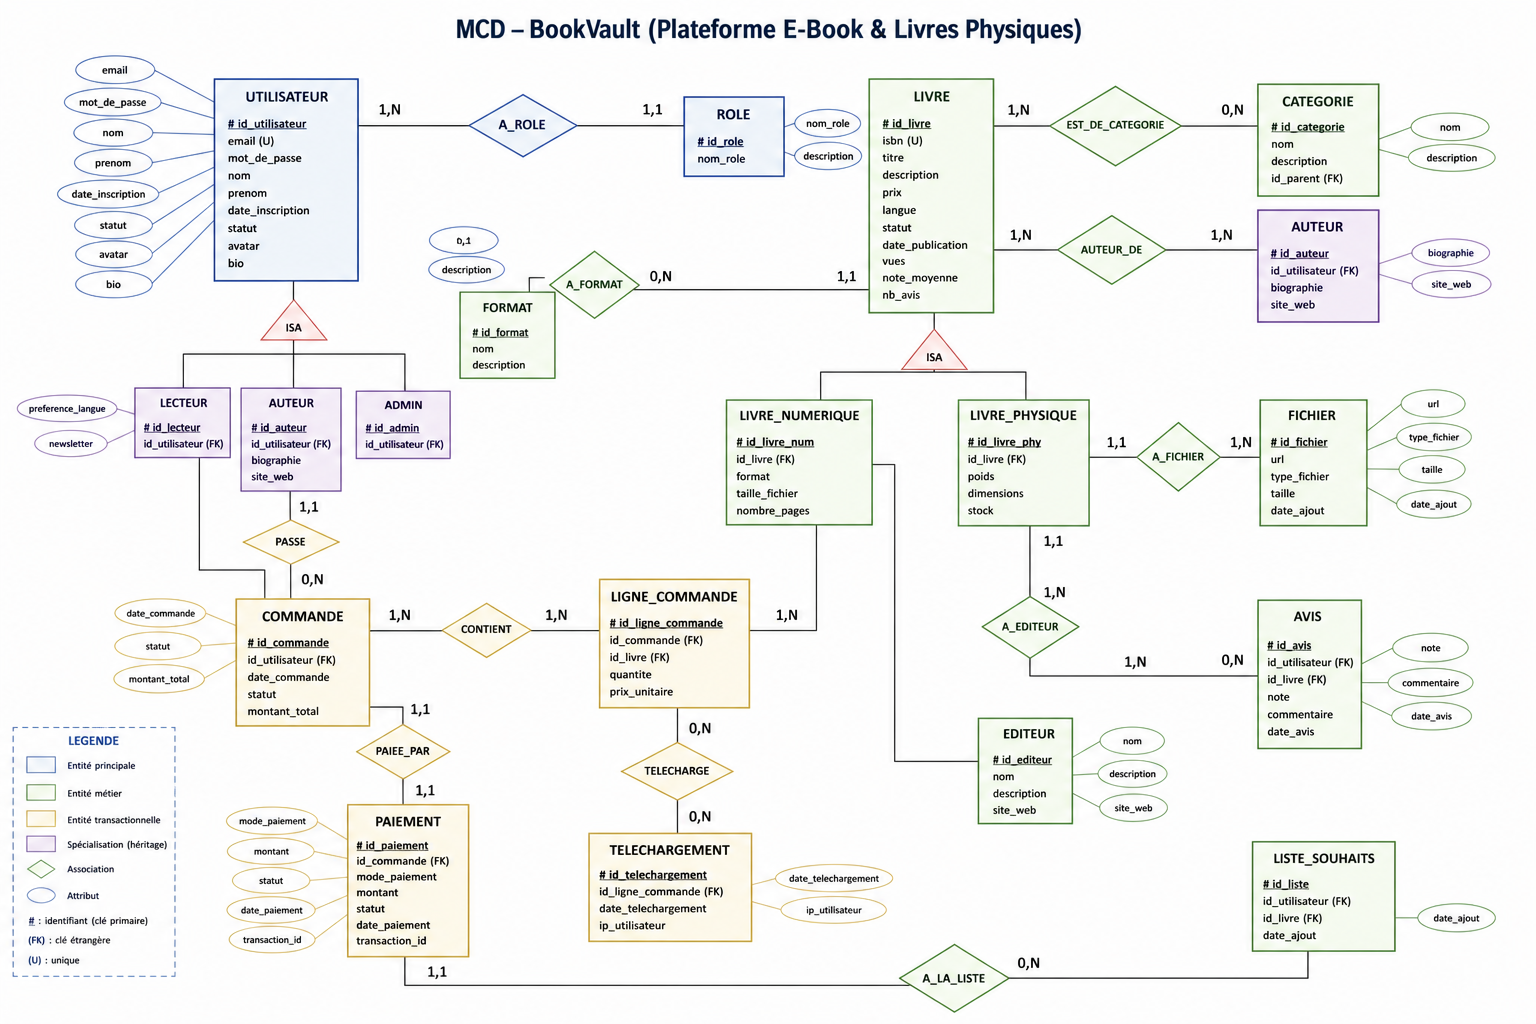
\includegraphics[width=0.92\textwidth]{bukvault-MCD.png}
  \caption{Modèle conceptuel de données BookVault (entités et relations métier).}
  \label{fig:mcd}
\end{figure}

\section{Communication inter-services et cohérence}
Les fiches théoriques correspondantes (HTTP synchrone, CAP, Kafka, BFF, Saga, Outbox) sont au chapitre~\ref{ch:referentiel}.

\subsection{Appels synchrones HTTP (approche actuelle)}
Les intégrations reposent sur des clients HTTP configurables : \textit{order-service} interroge \textit{catalog-service} ; \textit{file-service} et \textit{reading-service} vérifient les droits via \textit{order-service} ; \textit{wishlist-service} transfère vers le panier ; \textit{admin-service} agrège plusieurs backends. Ce modèle est simple à déboguer mais introduit latence cumulée et dépendances au moment de l'exécution.\par

\subsection{Cohérence et compromis (théorie distribuée)}
Dans un système distribué, le théorème CAP rappelle qu'on ne peut pas garantir simultanément cohérence forte, disponibilité et tolérance au partitionnement. BookVault privilégie la \textbf{disponibilité} et la \textbf{séparation des domaines}, avec une cohérence \textbf{éventuelle} sur certains agrégats (notes moyennes, compteurs de vues, dashboards admin). Les stubs et endpoints internes permettent de contourner temporairement l'absence d'un service partenaire en développement.\par

\subsection{Événements asynchrones (perspective)}
Une évolution classique publierait des événements (\texttt{OrderPaid}, \texttt{BookPublished}) via \textbf{Kafka} ou RabbitMQ, découplant producteurs et consommateurs et permettant des traitements différés (e-mails, stats, caches). Le \textbf{pattern Outbox} garantirait la fiabilité de ces publications, et le pattern \textbf{Saga} gérerait les transactions multi-services (checkout, paiement, entitlements). Cette couche constitue une extension intergiciel naturelle du projet.\par

\subsection{Façade admin (pattern BFF)}
\textit{admin-service} agit comme \textbf{Backend For Frontend} : il orchestre des appels vers user, catalog, reading et review sans dupliquer la logique métier, produisant un tableau de bord unique pour l'administrateur.\par

\section{Réseau distribué}
En démonstration multi-postes, la gateway accepte des URIs pointant vers des machines distantes (\texttt{AUTH\_SERVICE\_URI=http://192.168.x.x:8081}). Le front cible l'IP de la machine hébergeant la gateway. Les enjeux incluent pare-feu, partage du \texttt{JWT\_SECRET} entre resource servers, et configuration CORS.\par

% =========================================================
% 4. Technologies
% =========================================================
\chapter{Technologies et choix d'implémentation}
\section{Backend (Spring Boot)}
\subsection{Spring Boot + JPA + PostgreSQL}
Chaque microservice est un projet Maven Spring Boot autonome. La persistance repose sur JPA (Hibernate) et PostgreSQL. Le choix est motivé par la maturité de l'écosystème, la facilité d'exposer des DTOs (`record` Java), et le support de migrations évolutives.\par

\subsection{Spring Security : Resource Server}
Les services (hors auth) se comportent comme \textbf{Resource Servers} : ils valident les JWT et appliquent des règles RBAC (USER/AUTHOR/ADMIN). L'auth-service est l'émetteur des tokens.\par

\section{Frontend (Angular)}
Le client Angular consomme l'API via `/api/v1` (proxy en développement). Il implémente l'état d'authentification (JWT + refresh), la navigation par rôle (guards), l'intégration Google (GIS), et une UX cohérente autour des notifications (cloche) et des parcours d'inscription/vérification e-mail.\par

\section{API Gateway et configuration}
(Voir fiche API Gateway, chapitre~\ref{ch:referentiel}.) L'API Gateway joue le rôle d'intergiciel « frontal » : point d'entrée unique, routage vers les microservices, et gestion du CORS pour le front Angular. Le front utilise un proxy local afin de simplifier les URLs et d'éviter les problèmes d'origine en environnement de développement.\par

\section{Outils et déploiement local}
\begin{itemize}
  \item \textbf{Docker Compose} : orchestration locale des bases PostgreSQL et services.
  \item \textbf{Scripts SQL de seed} : jeux de démonstration reproductibles (comptes, catalogue, commandes).
  \item \textbf{Variables d'environnement} : configuration des URIs inter-services via la gateway (\texttt{AUTH\_SERVICE\_URI}, etc.).
\end{itemize}

% =========================================================
% 5. Sécurité & Auth
% =========================================================
\chapter{Sécurité, authentification et conformité}

Les fiches JWT, OAuth/OIDC, RBAC et Resource Server sont au chapitre~\ref{ch:referentiel}. Ci-dessous : mise en œuvre BookVault.

\section{JWT : access + refresh}
L'auth-service délivre un access token (court) et un refresh token stocké. Les refresh permettent la rotation et l'invalidation. Un mécanisme de blacklist de jti supporte le logout.\par

\section{Diagramme de séquence — authentification et inscription}
\label{sec:diagramme-seq-auth}

L'ébauche ci-dessous modélise les échanges entre l'utilisateur, le front Angular, l'API Gateway et les microservices \textit{auth-service} et \textit{notification-service} lors de l'\textbf{inscription} (création de compte, envoi du lien de vérification) et de la \textbf{connexion} (délivrance des tokens JWT). Elle illustre le rôle de l'intergiciel : un point d'entrée unique (\texttt{/api/v1}) et des services métier spécialisés en aval.\par

\textbf{Acteurs et composants représentés :}
\begin{itemize}
  \item \textbf{Utilisateur} : saisie du formulaire d'inscription ou de connexion ;
  \item \textbf{Angular} (\texttt{AuthService}, intercepteur HTTP) : appels API, stockage des tokens ;
  \item \textbf{API Gateway} : routage vers \textit{auth-service} ;
  \item \textbf{auth-service} : validation, hachage BCrypt, émission JWT / refresh ;
  \item \textbf{notification-service} : envoi du message de vérification e-mail (appel interne).
\end{itemize}

\textbf{Fichier à insérer :} placer \texttt{flux\_inscription\_utilisateur.png} dans le même dossier que ce document (Overleaf ou compilation locale).\par

\begin{figure}[H]
  \centering
  \IfFileExists{flux_inscription_utilisateur.png}{%
    \includegraphics[width=0.95\textwidth]{flux_inscription_utilisateur.png}%
  }{%
    \fbox{%
      \parbox{0.88\textwidth}{%
        \centering\vspace{2.8cm}
        \textbf{Ébauche — diagramme de séquence}\\[0.6em]
        \textit{Authentification / inscription utilisateur}\\[0.8em]
        Fichier attendu : \texttt{flux\_inscription\_utilisateur.png}\\[0.4em]
        (même répertoire que \texttt{Intergiciel\_Rapport\_BukVault.tex})
        \vspace{2.8cm}%
      }%
    }%
  }%
  \caption{Ébauche de diagramme de séquence — flux d'inscription et d'authentification utilisateur (Angular, gateway, auth-service, notification-service). Source : \texttt{flux\_inscription\_utilisateur.png}.}
  \label{fig:flux-inscription-utilisateur}
\end{figure}

\section{OAuth Google (GIS) et vérification e-mail}
La connexion Google s'appuie sur Google Identity Services côté front, et sur une validation du \textit{id\_token} côté back. Pour la sécurité, le token de vérification e-mail est un JWT dédié (purpose=email\_verify) signé HMAC et expirant sous 24h. Cette stratégie évite la gestion d'un simple UUID non authentifié.\par

\section{Protection des endpoints internes}

Les endpoints \texttt{/internal/**} (entitlements, agrégations) ne sont appelés que par d'autres services et ne doivent jamais être exposés à Internet. Plusieurs niveaux de protection sont applicables :

\begin{itemize}
  \item \textbf{Isolation réseau} : en production, les services backend communiquent sur un réseau privé (VPC, réseau Docker interne) inaccessible de l'extérieur. La gateway ne route pas les chemins \texttt{/internal/**} vers l'extérieur.
  \item \textbf{Clé API de service} (\textit{service API key}) : chaque appel interne inclut un en-tête \texttt{X-Internal-Api-Key} partagé entre services de confiance, validé par un filtre Spring Security dédié.
  \item \textbf{mTLS inter-services} : en environnement Kubernetes avec Istio/Linkerd, les sidecars gèrent automatiquement des certificats mutuels, garantissant que seul un service authentifié peut appeler un autre. Transparent pour le code applicatif.
  \item \textbf{Scopes JWT dédiés} : les tokens inter-services peuvent contenir un claim \texttt{client\_id} ou \texttt{scope=internal} refusé pour les tokens utilisateur finaux.
\end{itemize}

BookVault V1 s'appuie sur l'isolation réseau Docker Compose et l'absence de route gateway vers \texttt{/internal}. Un durcissement progressif vers les clés API de service est recommandé avant toute exposition publique.

\section{Rotation des secrets et gestion des credentials}

Dans un système distribué, la gestion du \texttt{JWT\_SECRET} partagé entre tous les resource servers est un point de fragilité. Bonnes pratiques :

\begin{itemize}
  \item \textbf{HashiCorp Vault ou AWS Secrets Manager} : les secrets ne sont jamais hardcodés ni committés dans le dépôt. Chaque service les lit au démarrage depuis un gestionnaire de secrets avec TTL et audit.
  \item \textbf{Rotation sans interruption} : utiliser \textbf{RSA (RS256)} plutôt que HMAC partagé (HS256) permet à chaque service de ne disposer que de la \textbf{clé publique} pour vérifier les tokens. La clé privée reste dans auth-service. La rotation ne nécessite alors que de mettre à jour la clé privée dans auth-service et de publier la nouvelle clé publique via l'endpoint JWKS (\texttt{/.well-known/jwks.json}).
  \item \textbf{Durée de vie courte des tokens} : access tokens de 15 minutes maximum réduit la fenêtre d'exploitation en cas de fuite.
\end{itemize}

\section{Stratégies de contournement (dev) et optimisation}
Dans un système distribué, certaines dépendances externes peuvent ralentir le développement (paiement, entitlement, stockage réel). Le projet implémente des stratégies :
\begin{itemize}
  \item \textbf{Stubs d'entitlements} : file-service et reading-service peuvent fonctionner sans order-service en dev (flags de configuration).
  \item \textbf{Migration progressive} : ajout de colonnes auth (provider Google, emailVerified) via JPA update pour éviter un blocage en environnement étudiant.
  \item \textbf{Proxy Angular} : correction des appels vers le gateway (évite le routage erroné vers :4200).
  \item \textbf{Notification "session expirée"} : UX améliorée en remplaçant un bandeau intrusif par une notification persistante.
\end{itemize}

% =========================================================
% 6. Détails d'implémentation (microservices + frontend)
% =========================================================
\chapter{Détails d'implémentation : microservices et frontend}

\section{Contrats API (DTO) et stabilité}
Le backend expose des DTOs sous forme de \textit{records} Java (ex. \texttt{UserResponse}, \texttt{BookDetailResponse}). Ce choix force une \textbf{surface d'API explicite} et stable : seuls les champs du DTO sont sérialisés, ce qui limite les fuites de modèle interne et simplifie l'évolution.\par

\section{Catalogue (\textit{catalog-service})}
\subsection{Ressources et statuts}
Le service catalogue gère :
\begin{itemize}
  \item les livres (\texttt{id}, \texttt{isbn}, \texttt{title}, \texttt{description}, \texttt{price}, \texttt{language}, \texttt{format}, \texttt{status});
  \item les catégories hiérarchiques (slug, ordre d'affichage);
  \item la visibilité : un livre \texttt{PUBLISHED} et non supprimé est visible publiquement, tandis que les brouillons sont réservés à l'auteur/admin.\par
\end{itemize}

\subsection{Technique : séparation public / auteur}
Un point important est la distinction entre les listes publiques et la vue « auteur ». Le projet introduit un endpoint dédié (\texttt{/books/mine}) qui renvoie \textbf{tous les statuts} pour l'utilisateur authentifié, évitant un comportement où \texttt{/books} ne retourne que les livres publiés.\par

\section{Commandes et panier (\textit{order-service})}
\subsection{Panier persistant et commandes}
Le panier est persistant par utilisateur (\textit{cart lines}). Lors du checkout, une commande (\textit{order}) est créée avec ses lignes. Le service expose également un endpoint interne d'entitlements utilisé par d'autres services.\par

\subsection{Technique : entitlements internes}
(Voir fiche « Entitlements », chapitre~\ref{ch:referentiel}.) Les services \textit{file-service} et \textit{reading-service} ne doivent pas ré-implémenter la logique d'accès. Ils interrogent \textit{order-service} via un endpoint interne (\texttt{/internal/entitlements/...}) renvoyant \texttt{allowed}. Cela respecte la séparation des responsabilités et évite les dépendances directes à la base des commandes.\par

\section{Fichiers (\textit{file-service})}
\subsection{Kinds et stockage}
Le service fichiers gère les uploads et downloads et stocke des métadonnées (\texttt{stored\_file}). Chaque fichier a un \texttt{kind} (\texttt{EBOOK}, \texttt{COVER}, \texttt{AVATAR}), un \texttt{storageKey}, un \texttt{mimeType} et une \texttt{sizeBytes}. Les objets sont adressés via des routes dédiées (ex. download ebook).\par

\subsection{Technique : contrôle d'accès en amont du download}
Avant de servir un ebook, le service vérifie l'accès via \textit{order-service}. En développement, un mode \textbf{stub} est disponible pour ne pas bloquer les tests end-to-end lorsque l'interconnexion n'est pas activée.\par

\section{Lecture (\textit{reading-service})}
La progression de lecture est stockée sous forme d'un identifiant composite (\texttt{userId}, \texttt{bookId}, \texttt{mediaType}) et d'un champ \texttt{positionJson} libre. Cela permet de supporter des stratégies multiples (page, pourcentage, offset EPUB, secondes audio) sans multiplier les colonnes.\par

\section{Avis (\textit{review-service})}
Le service avis maintient :
\begin{itemize}
  \item les avis (note, titre, corps, achat vérifié) ;
  \item le compteur \texttt{helpfulCount} et l'état \texttt{markedByMe} ;
  \item les signalements avec raison (\texttt{SPAM}, \texttt{OFFENSIVE}, etc.).\par
\end{itemize}
Ces éléments alimentent la modération (open reports) et la qualité perçue.\par

\section{Notifications (\textit{notification-service})}
Les préférences de notification (email/in-app/marketing) et les notifications applicatives sont séparées. Côté front, l'événement « session expirée » a été déplacé vers la cloche de notifications afin d'éviter un bandeau intrusif.\par

\section{Frontend Angular : structure et flux}
\subsection{Organisation}
Le front est organisé par pages (auth, reader dashboard, author dashboard) et services (auth, books, notifications). Les types d'API sont centralisés pour limiter les divergences de champs.\par

\subsection{Flux d'authentification}
Les parcours décrits ici correspondent au diagramme de séquence (figure~\ref{fig:flux-inscription-utilisateur}, section~\ref{sec:diagramme-seq-auth}).\par
\begin{itemize}
  \item Connexion classique : login → réception tokens → stockage + expiration → refresh automatique.
  \item Connexion Google : récupération \texttt{idToken} via GIS, puis \texttt{POST /auth/google}.
  \item Vérification e-mail : l'API peut renvoyer \texttt{emailVerificationRequired} (sans tokens), redirection vers pages de vérification.\par
\end{itemize}

\subsection{Espace auteur : opérations sur les livres}
L'interface auteur affiche les livres de l'auteur (tous statuts) via \texttt{/books/mine} et propose des actions selon l'état :
soumettre à validation, publier/retirer, supprimer. Cette logique côté UI reflète strictement les règles RBAC et les endpoints du backend.\par

\section{Wishlist, communauté, auteur et administration}
\subsection{Wishlist (\textit{wishlist-service})}
Liste de favoris par utilisateur ; transfert vers panier via appel HTTP vers \textit{order-service} en propageant le JWT. Pattern « orchestration légère » côté service appelant.\par

\subsection{Communauté (\textit{community-service})}
Hub, fils de discussion, événements, messagerie directe, likes livre et suggestions de lecteurs (« buddies »). Modèle social distinct du catalogue transactionnel.\par

\subsection{Auteur et admin}
\textit{author-service} expose le profil public (nom de plume, bio) et des stats ; \textit{admin-service} agrège KPI, courbes de lecture et signalements pour la modération.\par

% =========================================================
% 7. Techniques API et contrats REST
% =========================================================
\chapter{Techniques API, validation et documentation}

Les définitions de REST, DTO, pagination, OpenAPI, idempotence et HATEOAS figurent au chapitre~\ref{ch:referentiel}. Ce chapitre détaille leur \textbf{application} dans BookVault.

\section{Principes REST et versionnement}
Toutes les ressources publiques sont préfixées par \texttt{/api/v1}, ce qui permet une évolution future (\texttt{v2}) sans casser les clients existants. Les verbes HTTP respectent les sémantiques REST : \texttt{GET} lecture, \texttt{POST} création, \texttt{PUT/PATCH} mise à jour, \texttt{DELETE} suppression logique ou physique selon le domaine.\par

\section{DTOs, validation et séparation des couches}
Les contrôleurs reçoivent des \textbf{requêtes validées} (\texttt{@Valid}, contraintes Jakarta Bean Validation) et renvoient des \textbf{DTOs} (\texttt{record} Java) plutôt que des entités JPA. Cette séparation évite l'exposition accidentelle de champs internes (hash mot de passe, relations lazy Hibernate) et stabilise le contrat consommé par Angular.\par

\section{Pagination et filtrage}
Les listes (utilisateurs, livres, commandes, notifications) s'appuient sur \texttt{Pageable} Spring Data : paramètres \texttt{page}, \texttt{size}, \texttt{sort}. La réponse inclut \texttt{content}, \texttt{totalElements}, \texttt{totalPages}, ce qui permet au front de paginer sans charger des milliers d'enregistrements.\par

\section{Gestion des erreurs}
Une stratégie centralisée (\texttt{@ControllerAdvice}) normalise les réponses d'erreur (400 validation, 401 non authentifié, 403 interdit, 404 introuvable, 409 conflit, 500 serveur). Le front peut ainsi afficher des messages cohérents plutôt que parser des stacks techniques.\par

\section{Documentation OpenAPI}
Chaque microservice peut exposer Swagger UI (springdoc-openapi), documentant chemins, schémas de requête/réponse et codes HTTP. Cela sert de contrat vivant entre équipes front et back.\par

\section{Endpoints internes vs publics}
Certains chemins (\texttt{/internal/entitlements/...}) sont réservés au réseau de confiance inter-services. En production, ils seraient protégés par réseau privé, mTLS ou clé API de service — technique de durcissement non obligatoire en démonstration locale.\par

\section{Techniques d'API non encore déployées (extensions possibles)}
\begin{itemize}
  \item \textbf{HATEOAS} : liens hypermédia dans les réponses pour découvrabilité des actions suivantes.
  \item \textbf{Idempotency-Key} sur \texttt{POST /orders} et paiements pour éviter les doubles commandes en cas de retry réseau.
  \item \textbf{Rate limiting} à la gateway (token bucket, Redis) contre les abus.
  \item \textbf{Circuit breaker / retry} (Resilience4j) sur les appels inter-services.
  \item \textbf{GraphQL ou gRPC} pour réduire le nombre d'allers-retours sur des écrans complexes (non retenu : REST suffit pour la V1).
  \item \textbf{Webhooks signés} (HMAC) pour les PSP réels au lieu du stub actuel.
  \item \textbf{Consumer-Driven Contract Testing} (Pact) pour sécuriser les évolutions de contrats API entre services.
\end{itemize}

% =========================================================
% 8. Frontend Angular — architecture détaillée
% =========================================================
\chapter{Frontend Angular : architecture et intégration}

(Voir fiche « Proxy, intercepteur, guards », chapitre~\ref{ch:referentiel}.)

\section{Organisation modulaire}
L'application est découpée en pages lazy-loaded (accueil, catalogue, auteur, lecteur, auth), services injectables (\texttt{AuthService}, \texttt{BookService}, \texttt{CartService}) et modèles TypeScript alignés sur les DTOs Java (\texttt{api.types.ts}). Cette homogénéisation limite les écarts de nommage entre front et back.\par

\section{Proxy, intercepteur et état d'authentification}
En développement, \texttt{proxy.conf.json} redirige \texttt{/api/v1} vers la gateway (port 8080). Un intercepteur HTTP ajoute automatiquement \texttt{Authorization: Bearer} sauf sur login/register/refresh. Les tokens sont stockés côté client ; un coordinateur gère le refresh et la déconnexion en cas d'expiration.\par

\section{Guards et RBAC côté UI}
Les routes protégées utilisent des guards Angular vérifiant le rôle (\texttt{USER}, \texttt{AUTHOR}, \texttt{ADMIN}) avant d'activer un dashboard. Cela duplique partiellement le RBAC serveur (défense en profondeur) : le serveur reste l'autorité finale.\par

\section{Parcours utilisateur couverts}
\begin{itemize}
  \item Inscription / connexion classique et Google (GIS).
  \item Vérification e-mail (pages dédiées, pas de JWT tant que non vérifié).
  \item Catalogue public, fiche livre, panier, espace auteur (\texttt{/books/mine}).
  \item Notifications (cloche) incluant session expirée.
\end{itemize}

\section{Techniques front non encore généralisées}
\begin{itemize}
  \item Intercepteur 401 $\rightarrow$ refresh automatique puis retry systématique.
  \item State management global (NgRx) si la complexité augmente.
  \item Lecteur intégré branché sur \texttt{reading-service} et URLs signées \texttt{file-service}.
  \item Checkout complet (\texttt{POST /orders}, paiement) depuis le panier.
  \item Internationalisation (i18n) et accessibilité renforcée (ARIA).
\end{itemize}

% =========================================================
% 9. Sécurité approfondie
% =========================================================
\chapter{Sécurité : mécanismes et bonnes pratiques}

Ce chapitre complète le chapitre~\ref{ch:referentiel} (fiches JWT, OAuth, RBAC) par des détails d'implémentation et de durcissement.

\section{Hachage des mots de passe}
BCrypt (force 12) pour les comptes locaux ; les comptes Google utilisent un hash aléatoire non utilisable pour la connexion locale, forçant le flux OAuth.\par

\section{Structure du JWT}
Claims typiques : \texttt{sub} (UUID utilisateur), \texttt{email}, \texttt{role}. Signature HS256 avec secret partagé (\texttt{JWT\_SECRET}) entre auth-service et resource servers. Durée de vie courte pour l'access token ; refresh opaque stocké hashé en base.\par

\section{Révocation et logout}
Blacklist des \texttt{jti} des access tokens ; révocation des refresh tokens (un jeton ou tous). Permet une déconnexion effective même si l'access token n'est pas encore expiré.\par

\section{OAuth 2.0 / OpenID Connect}
Le front obtient un \texttt{id\_token} Google ; le back le valide (audience, émetteur) avant de créer ou lier le compte. Évite de gérer le mot de passe Google côté serveur.\par

\section{Durcissements futurs}
HTTPS obligatoire en production, rotation des secrets (voir section dédiée au chapitre précédent), mTLS inter-services (Istio/Linkerd), WAF, audit des dépendances (OWASP Dependency Check), limitation des tentatives de login (Bucket4j), CSP côté front.\par

% =========================================================
% 10. Persistance, fichiers et intégrations externes
% =========================================================
\chapter{Persistance, stockage et intégrations}

\section{JPA et stratégie de schéma}
Hibernate mappe les entités ; en développement, \texttt{ddl-auto=update} accélère l'itération. En production, Flyway/Liquibase serait préférable pour des migrations versionnées et reproductibles.\par

\section{Stockage fichiers}
Métadonnées en PostgreSQL (\texttt{stored\_file}) ; binaires sur disque local (\texttt{file.storage.root}). Évolution naturelle : \textbf{MinIO} ou S3 avec URLs pré-signées pour scaler et externaliser le stockage.\par

\section{Paiement et e-mail}
Le paiement est simulé (\texttt{POST .../pay}) avec référence type Mobile Money camerounaise. Une intégration Stripe/PayPal nécessiterait webhooks signés et gestion d'idempotence. Les e-mails (vérification, reset password) passent par \textit{notification-service} en appel interne ; SMTP/SendGrid reste une brique externe classique.\par

% =========================================================
% 11. Qualité, observabilité et déploiement
% =========================================================
\chapter{Qualité logicielle, observabilité et déploiement}

\section{Tests}
Tests unitaires sur services critiques (auth, catalogue, commandes) ; tests d'intégration avec Testcontainers PostgreSQL pour valider les repositories. Le front peut mocker les services HTTP (Jasmine) pour tester les composants isolément.\par

\section{Consumer-Driven Contract Testing}
En complément des tests unitaires et d'intégration, les tests de contrat consommateur (Pact) constituent une pratique clé en environnement microservices : ils détectent les régressions d'API \textit{avant} déploiement, sans orchestrer l'ensemble du système. Applicable sur les paires \textit{order-service} $\leftrightarrow$ \textit{catalog-service} et \textit{Angular} $\leftrightarrow$ \textit{auth-service} (voir fiche dédiée au chapitre~\ref{ch:referentiel}).\par

\section{Observabilité (extensions)}
Logs structurés (JSON), corrélation des requêtes (\texttt{X-Request-Id} propagé par la gateway), métriques Prometheus + Grafana, traces distribuées (OpenTelemetry + Zipkin/Jaeger). Le tracing distribué est particulièrement précieux pour diagnostiquer les latences cumulées des appels inter-services (voir fiche Distributed Tracing au chapitre~\ref{ch:referentiel}).\par

\section{Docker et orchestration}
Docker Compose lance bases et services ; variables d'environnement injectent les URIs. Les \textbf{healthchecks} Docker Compose garantissent l'ordre de démarrage correct (PostgreSQL avant services JPA). Kubernetes serait l'étape suivante (ConfigMaps, Secrets, Ingress, HPA, readiness/liveness probes natives).\par

% =========================================================
% 12. Résultats et discussion
% =========================================================
\chapter{Résultats, validation et discussion}
\section{Fonctionnel}
Les parcours principaux (auth, catalogue, commandes, lecture, avis, wishlist, notifications, communauté) sont considérés \textbf{implémentés et validés}. Les écrans auteur (gestion du cycle de vie d'un livre) et les endpoints associés permettent soumission, publication, retrait, suppression.\par

\section{Qualité et maintenabilité}
La séparation des domaines, l'usage de DTOs explicites, et la standardisation `/api/v1` rendent l'ensemble maintenable. Les configurations par variables d'environnement facilitent l'exécution locale et en conteneurs.\par

\section{Performance et scalabilité}
Le design favorise l'évolutivité :
\begin{itemize}
  \item \textbf{Scaling horizontal} : services fortement sollicités (catalog, file, order) peuvent être répliqués.
  \item \textbf{Réduction des couplages} : les services consultent des API internes au lieu d'accéder directement à des tables d'un autre domaine.
  \item \textbf{Limitation du couplage front/back} : DTOs explicites, proxy `/api/v1`, erreurs centralisées côté UI.
\end{itemize}

% =========================================================
% 13. Conclusion
% =========================================================
\chapter{Conclusion}
BookVault illustre une approche intergiciel moderne : une plateforme distribuée modulaire, sécurisée, observable et extensible. Les microservices réduisent le couplage, améliorent l'agilité et clarifient les responsabilités. Les stratégies de stubs, la gestion des tokens (JWT, vérification e-mail), et les optimisations UX (notifications) montrent comment une architecture distribuée se construit pragmatiquement.\par
\par
Au final, l'architecture permet d'ajouter ou de modifier des domaines (lecture, communauté, administration) sans réécrire l'ensemble. La gateway, la sécurité partagée (JWT), et la séparation des bases par service constituent le cœur intergiciel de la solution. Les patterns avancés documentés dans ce rapport (Saga, Outbox, Service Discovery, Distributed Tracing, Contract Testing) dessinent la feuille de route naturelle d'une montée en maturité vers un système de production robuste.\par

% =========================================================
% Bibliographie (sources des fiches théoriques)
% =========================================================
\chapter*{Bibliographie sélective}
\addcontentsline{toc}{chapter}{Bibliographie sélective}
\begin{itemize}
  \item BookVault, Votre Marketplace Littéraire. (2026). \textit{Projet d'intergiciel}. \url{https://github.com/Asaph-D/bukvault.git}
  \item Brewer, E. A. (2000). \textit{Towards Robust Distributed Systems} (théorème CAP). Preuve formelle : Gilbert, S., \& Lynch, N. (2002).
  \item Fielding, R. T. (2000). \textit{Architectural Styles and the Design of Network-based Software Architectures} (REST). UC Irvine.
  \item Fowler, M., \& Lewis, J. (2014). \textit{Microservices}. \url{https://martinfowler.com/articles/microservices.html}
  \item Fowler, M. (2014). \textit{Circuit Breaker}. \url{https://martinfowler.com/bliki/CircuitBreaker.html}
  \item IETF RFC 6749 (OAuth 2.0), RFC 7519 (JWT), RFC 9068 (JWT access tokens).
  \item OpenID Connect Core 1.0. \url{https://openid.net/specs/openid-connect-core-1_0.html}
  \item Newman, S. \textit{Building Microservices} ; pattern BFF (Microsoft Azure Architecture Center).
  \item NIST — RBAC (ANSI/INCITS 359). \url{https://csrc.nist.gov/projects/role-based-access-control}
  \item MDN Web Docs — CORS. \url{https://developer.mozilla.org/en-US/docs/Web/HTTP/Guides/CORS}
  \item microservices.io — Database per service, Idempotent consumer, Saga, Transactional Outbox.
  \item Microsoft Learn — API Gateway, Circuit Breaker, Backends for Frontends.
  \item Richardson, C. (2018). \textit{Microservices Patterns}. Manning Publications.
  \item W3C Trace Context Recommendation. \url{https://www.w3.org/TR/trace-context/}
  \item OpenTelemetry — \url{https://opentelemetry.io/docs/}
  \item Pact Foundation — \url{https://docs.pact.io/}
  \item Debezium — Change Data Capture. \url{https://debezium.io/documentation/}
  \item Netflix Eureka — \url{https://github.com/Netflix/eureka}
  \item Spring Boot Actuator Reference. \url{https://docs.spring.io/spring-boot/docs/current/reference/html/actuator.html}
\end{itemize}

% =========================================================
% Annexes
% =========================================================

\chapter{Exemples d'appels API (extraits)}
\section{Exemple : profil utilisateur}
\begin{lstlisting}[caption={GET /api/v1/auth/me (réponse)},label={lst:authme}]
{
  "id": "550e8400-e29b-41d4-a716-446655440000",
  "email": "marie.essama@users.cm",
  "firstName": "Marie",
  "lastName": "Essama",
  "role": "USER",
  "active": true,
  "emailVerified": true,
  "createdAt": "2026-05-01T10:30:00Z"
}
\end{lstlisting}

\section{Exemple : livre (détail)}
\begin{lstlisting}[caption={GET /api/v1/books/{id} (réponse)},label={lst:bookdetail}]
{
  "id": "660e8400-e29b-41d4-a716-446655440001",
  "title": "APC 3ème : cours & exercices",
  "isbn": "9782372510104",
  "description": "Manuel APC — révisions et exercices.",
  "price": 7.50,
  "language": "fr",
  "format": "EBOOK",
  "status": "PUBLISHED",
  "authorId": "20000000-0000-4000-a000-000000000006",
  "coverUrl": null,
  "averageRating": 4.2,
  "reviewCount": 9,
  "viewCount": 9100,
  "deleted": false,
  "publishedAt": "2026-01-10T00:00:00Z",
  "createdAt": "2025-12-01T08:00:00Z",
  "updatedAt": "2026-05-01T12:00:00Z",
  "categories": [{ "id": "e0000005-0000-4000-8000-000000000005",
                   "name": "Scolaire (APC)", "slug": "scolaire-apc" }]
}
\end{lstlisting}

\section{Exemple : entitlement interne}
\begin{lstlisting}[caption={GET /api/v1/internal/entitlements/users/\{userId\}/books/\{bookId\}},label={lst:entitlement}]
{
  "userId": "550e8400-e29b-41d4-a716-446655440000",
  "bookId": "660e8400-e29b-41d4-a716-446655440001",
  "allowed": true,
  "reason": "ORDER_PAID"
}
\end{lstlisting}

\chapter{Améliorations futur}

Cette annexe présente les étapes de transition vers une architecture de production plus robuste et classées par priorité.

\section{Étape 1 — Fiabilité de base (priorité haute)}
\begin{itemize}
  \item \textbf{Migrations de schéma versionnées} : remplacer \texttt{ddl-auto=update} par Flyway ou Liquibase sur chaque service. Garantit des migrations reproductibles, auditables et réversibles.
  \item \textbf{Health checks et dépendances Docker} : activer \texttt{spring-boot-starter-actuator} + \texttt{healthcheck} Docker Compose (\texttt{depends\_on: condition: service\_healthy}) pour éviter les race conditions au démarrage.
  \item \textbf{Secrets externalisés} : déplacer \texttt{JWT\_SECRET}, credentials PostgreSQL et clés API dans un gestionnaire de secrets (HashiCorp Vault, AWS Secrets Manager, ou variables Docker Secrets) plutôt qu'en clair dans \texttt{.env}.
  \item \textbf{HTTPS} : TLS terminé à la gateway (certificat Let's Encrypt ou load balancer cloud) pour chiffrer le trafic client.
\end{itemize}

\section{Étape 2 — Résilience (priorité moyenne)}
\begin{itemize}
  \item \textbf{Circuit breaker} (Resilience4j) sur les appels \textit{order} $\rightarrow$ \textit{catalog} et \textit{file} $\rightarrow$ \textit{order}. Configurer fallbacks (ex. retourner \texttt{allowed=false} si order-service est indisponible plutôt que de bloquer la requête).
  \item \textbf{Timeouts et retries avec backoff exponentiel} sur tous les appels HTTP inter-services.
  \item \textbf{Rate limiting} à la gateway (Redis + bucket4j ou Spring Cloud Gateway RateLimiter) pour protéger contre les abus.
  \item \textbf{Idempotency-Key} sur \texttt{POST /orders} et webhooks PSP.
\end{itemize}

\section{Étape 3 — Observabilité (priorité moyenne)}
\begin{itemize}
  \item \textbf{Distributed Tracing} : Micrometer Tracing + exporteur OTLP vers Zipkin ou Jaeger. Permet de diagnostiquer les latences cumulées en production.
  \item \textbf{Métriques} : Prometheus + Grafana pour surveiller les taux d'erreur, latences p99, saturation des pools de connexions PostgreSQL.
  \item \textbf{Logs structurés JSON} : Logback JSON encoder + agrégation ELK (Elasticsearch, Logstash, Kibana) ou Loki/Grafana.
\end{itemize}

\section{Étape 4 — Découplage événementiel (V2)}
\begin{itemize}
  \item \textbf{Kafka} : déployer un broker (Kafka + Zookeeper ou KRaft). Publier \texttt{OrderPaid}, \texttt{BookPublished}, \texttt{UserRegistered}.
  \item \textbf{Transactional Outbox} + Debezium CDC sur \texttt{bookvault\_order} pour garantir la publication fiable.
  \item \textbf{Saga par choreography} pour le flux checkout (réservation stock + paiement + confirmation).
  \item \textbf{Service Discovery} (Eureka ou Consul) pour éliminer les URIs statiques en production.
\end{itemize}

\section{Étape 5 — Orchestration Kubernetes}
\begin{itemize}
  \item Migration Docker Compose $\rightarrow$ Kubernetes (Deployments, Services, ConfigMaps, Secrets).
  \item Ingress NGINX ou Traefik remplaçant la gateway Spring Cloud Gateway (ou conservation de la gateway derrière l'Ingress).
  \item HPA (Horizontal Pod Autoscaler) sur catalog-service et order-service.
  \item Service mesh (Istio/Linkerd) pour mTLS automatique inter-services, circuit breaking et tracing sans modification du code.
\end{itemize}

\end{document}